% 
% Annual Cognitive Science Conference
% Sample LaTeX Paper -- Proceedings Format
% 

% Original : Ashwin Ram (ashwin@cc.gatech.edu)       04/01/1994
% Modified : Johanna Moore (jmoore@cs.pitt.edu)      03/17/1995
% Modified : David Noelle (noelle@ucsd.edu)          03/15/1996
% Modified : Pat Langley (langley@cs.stanford.edu)   01/26/1997
% Latex2e corrections by Ramin Charles Nakisa        01/28/1997 
% Modified : Tina Eliassi-Rad (eliassi@cs.wisc.edu)  01/31/1998
% Modified : Trisha Yannuzzi (trisha@ircs.upenn.edu) 12/28/1999 (in process)
% Modified : Mary Ellen Foster (M.E.Foster@ed.ac.uk) 12/11/2000
% Modified : Ken Forbus                              01/23/2004
% Modified : Eli M. Silk (esilk@pitt.edu)            05/24/2005
% Modified: Niels Taatgen (taatgen@cmu.edu) 10/24/2006

%% Change ``a4paper'' in the following line to ``letterpaper'' if you are
%% producing a letter-format document.

\documentclass[10pt,letterpaper]{article}

% uncomment below to put in cogsci format
%\usepackage{cogsci}

\usepackage{pslatex}
\usepackage{apacite}
\usepackage{amsmath}
\usepackage{graphicx}
\usepackage{color}
\usepackage{amssymb}

\usepackage{algorithmic}
\usepackage{algorithm}
\usepackage{amsthm}
\usepackage{float}
\usepackage{mathrsfs}
\usepackage{fullpage}


\newcommand{\footnoteremember}[2]{
\footnote{#2}
\newcounter{#1}
\setcounter{#1}{\value{footnote}}
}
\newcommand{\footnoterecall}[1]{
\footnotemark[\value{#1}]
}


%%%%%%%%%%%%%%%%%%%%%%%%%%%%%%%%%%%%%%%%%%%%%%%%%%%%%%%%%%%%%%%%%%%%%%
% title
%%%%%%%%%%%%%%%%%%%%%%%%%%%%%%%%%%%%%%%%%%%%%%%%%%%%%%%%%%%%%%%%%%%%%%
\title{{\bf VS265 Final Project}\\Exemplar storage in associative memory systems}
 
%%%%%%%%%%%%%%%%%%%%%%%%%%%%%%%%%%%%%%%%%%%%%%%%%%%%%%%%%%%%%%%%%%%%%%
% authors
%%%%%%%%%%%%%%%%%%%%%%%%%%%%%%%%%%%%%%%%%%%%%%%%%%%%%%%%%%%%%%%%%%%%%%
\author{{\large \bf Joshua T. Abbott (joshua.abbott@berkeley.edu)\footnoteremember{myfootnote}{The authors contributed equally to this work.}} \\
 {\large \bf Jessica B. Hamrick (jhamrick@berkeley.edu)\footnoterecall{myfootnote}} \\
% {\large \bf Thomas L. Griffiths (tom\_griffiths@berkeley.edu)} \\
  Department of Psychology, University of California, Berkeley, CA 94720 USA}

\date{}

\makeatletter
\@fpsep\textheight
\makeatother

\begin{document}

\maketitle

%%%%%%%%%%%%%%%%%%%%%%%%%%%%%%%%%%%%%%%%%%%%%%%%%%%%%%%%%%%%%%%%%%%%%%
% abstract
%%%%%%%%%%%%%%%%%%%%%%%%%%%%%%%%%%%%%%%%%%%%%%%%%%%%%%%%%%%%%%%%%%%%%%
\begin{abstract}
We explore the storage of exemplars in associative memory systems as an initial investigation into neural implementations of psychological processes. We first briefly outline a recent proposal that probabilistic models of cognition accounting for human behavior at a computational level of analysis can be approximated by existing psychological process models, namely, \textit{exemplar models}. Given this motivation, the main contribution of this paper consists of analyzing the dynamics and storage capabilities of two associative models of memory: a Hopfield network, and a Sparse Distributed Memory (SDM) system. We describe each model in a common mathematical framework and compare their performance  on storage capacity, retrieving prototypes, and retrieving sequences, using both corrupted and uncorrupted stimuli. Finding SDMs to be more robust and powerful computing machines, we then describe how the mechanics of SDMs can be interpreted probabilistically as a Monte Carlo method called importance sampling. We conclude with future directions of this research. 

% \textbf{Keywords:} 
% Sparse Distributed Memory systems, Bayesian inference, Exemplar model, Rational Process Model, Importance Sampling.
\end{abstract}

%%%%%%%%%%%%%%%%%%%%%%%%%%%%%%%%%%%%%%%%%%%%%%%%%%%%%%%%%%%%%%%%%%%%%%
% introduction
%%%%%%%%%%%%%%%%%%%%%%%%%%%%%%%%%%%%%%%%%%%%%%%%%%%%%%%%%%%%%%%%%%%%%%
\section{Introduction}

How do people make complicated inferences like separating concepts into categories, learning languages, or discovering causal relationships between events, constrained by limited evidence? Probabilistic models of cognition offer one such account of how people do this, with a rapidly growing body of literature supporting their claims \cite{griffiths2010probabilistic,tenenbaum2011grow}. These models provide a \textit{rational analysis} of human inductive inference, answering questions of cognition regarding \textit{why} people behave as they do \cite{marr82,anderson90}. However, traditional models from cognitive psychology focus on answering questions as to \textit{how} cognitive processes support these behaviors \cite{kahneman1972subjective,gigerenzer2000simple}. It remains unclear what psychological mechanisms could be responsible for carrying out the probabilistic computations in rational models. Furthermore, another line of research focuses on exploring ways to perform probabilistic computations with neural systems, providing answers to questions of cognition at Marr's level of \textit{implementation} \cite{ma2006bayesian}. In order to bridge these different methods of analyzing cognition, recent work has shown promise in using psychological process models as methods of approximating probabilistic inference \cite{Shi2010,sanborn2010rational,griffiths2012bridging} and using neural architectures to implement these computations \cite{Shi2009}. 

As motivation for our research, we focus on a particular investigation under this recent \textit{rational process model} approach, which uses an exemplar model of memory. It has been proposed that people store individual instances of observations in memory (as an \textit{exemplar}) and evaluate new observations by activating these exemplars as a function of their similarity to this novel event \cite{medin1978context,nosofsky1986attention}. \citeA{Shi2010} showed that this model of memory was formally equivalent to an importance sampler approximation of Bayesian inference. Here, the set of exemplars corresponds to a set of samples from a prior distribution. It has been further shown that this idea can be implemented with a Radial Basis Function (RBF) network \cite{Shi2009}. While this RBF implementation is an interesting proof-of-concept, it is not cognitively satisfying since each neuron in the model corresponds to a single exemplar; an extreme interpretation of the ``grandmother cell hypothesis''. In this paper, we set out to explore how exemplars are stored in associative models of memory as an alternative implementation of importance sampling. The plan of the paper is as follows. We first explore the mechanics behind two models of associative memory: a Hopfield network, and a Sparse Distributed Memory (SDM) system. We then analyze how well these models can store and retrieve patterns in memory. We then present how an SDM might perform importance sampling through a probabilistic interpretation of its read and write rules. Finally, we conclude the paper with our future directions for extending this research.


%%%%%%%%%%%%%%%%%%%%%%%%%%%%%%%%%%%%%%%%%%%%%%%%%%%%%%%%%%%%%%%%%%%%%%
% associative models of memory
%%%%%%%%%%%%%%%%%%%%%%%%%%%%%%%%%%%%%%%%%%%%%%%%%%%%%%%%%%%%%%%%%%%%%%
\section{Associative models of memory}

Associative models of memory comprise a set of information processing systems with the aim of storing and retrieving data by learning associations in the data. We consider two models in particular: a Hopfield network, and a Sparse Distributed Memory (SDM) system. We focus on these two models since Hopfield networks were covered in class; providing a foundation for which to compare to, and the mathematics between these two models has been previously presented in a unified framework \cite{Keeler1988}; allowing us to better understand the differences between each.  We present each model in a similar framework below. % For a more detailed exploration between these particular associative memory models, refer to \citeA{Keeler1988}, and for an alternative to SDMs that we do not explore (incorporating Hamming distance on binary patterns), please see \citeA{Lippmann1987}.

%%%%%%%%%%%%%%%%%%%%%%%%%%%%%%%%%%%%%%%%%%%%%%
% subsection - Hopfield networks
%%%%%%%%%%%%%%%%%%%%%%%%%%%%%%%%%%%%%%%%%%%%%%
\subsection{Hopfield networks}

Hopfield networks are an autoassociative model of memory, where a set of binary (+1/-1) patterns can be stored in the weights of a neural network and a pattern can be recovered from a noisy stimulus \cite{Hopfield1982}. More formally, given a set of binary patterns $\bf{p}^{\alpha}$ of length $N$, a symmetric $N \times N$ matrix $\bf{T}$ stores these patterns using the outer-product rule: $\bf{T} = \bf{T} + \bf{p}^{\alpha}\,\bf{p}^{\alpha\,'}$. To recover one of these stored patterns, a noisy input $\bf{x}$ is supplied to the network and a stochastic form of Hebbian learning is applied. For each  iteration $t$, a random output node $\bf{z}_{j}$ is selected and updated to (+1/-1) depending on the sign of $\sum_{j=1}^{N} \bf{T}_{ij}\,\bf{z}_{j}$. The Hopfield network architecture is depicted in panel (a) of Figure \ref{neuralNets} below.

While the Hopfield network has received popularity for its simplicity as a neural model of memory, a number of limitations have been posited in the literature \cite{Keeler1988}: (1) The storage capacity of a Hopfield network is bounded by a small fraction of the number of processing units - i.e., the length of the input; (2) they cannot handle temporal sequences of patterns; (3) the requirement of symmetric weights in $\bf{T}$ make Hopfield networks  implausible as a model of the brain; and (4) Hopfield networks have limited abilities to store correlated patterns. We explore a number of these concerns in Section 3, our analysis of exemplar storage in Hopfield networks and SDMs.

\begin{figure}[t!]
  \begin{center}
    \begin{tabular}{lclclc}
      \raisebox{1.6in}{(a)} &
      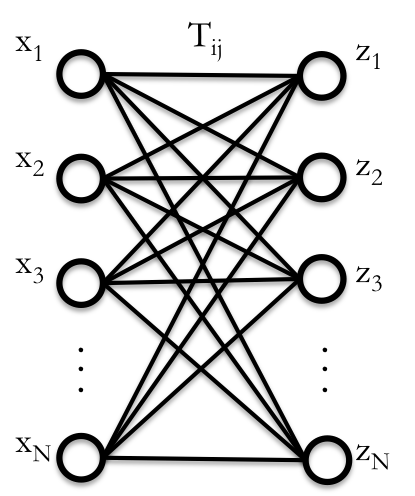
\includegraphics[width=0.23\textwidth]{./figures/hopfieldNetwork.png} &
      \raisebox{1.6in}{(b)} &
      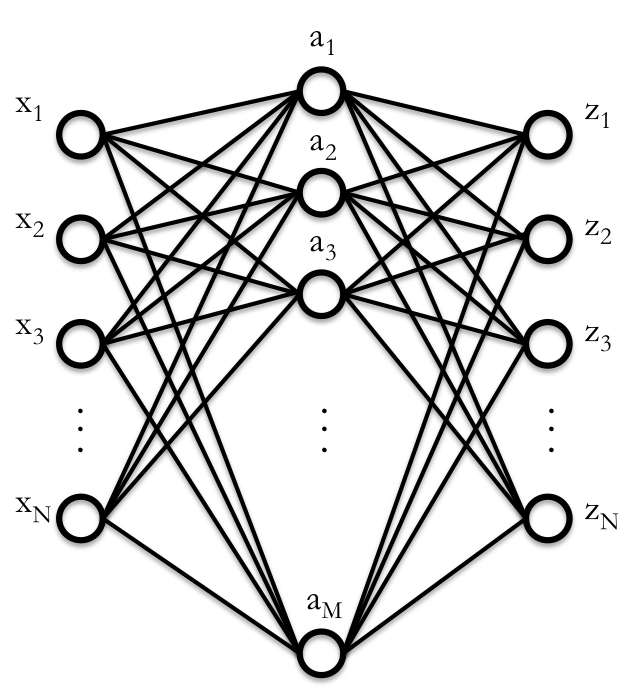
\includegraphics[width=0.27\textwidth]{./figures/sdmNetwork.png} 
      \raisebox{1.6in}{(c)} &
      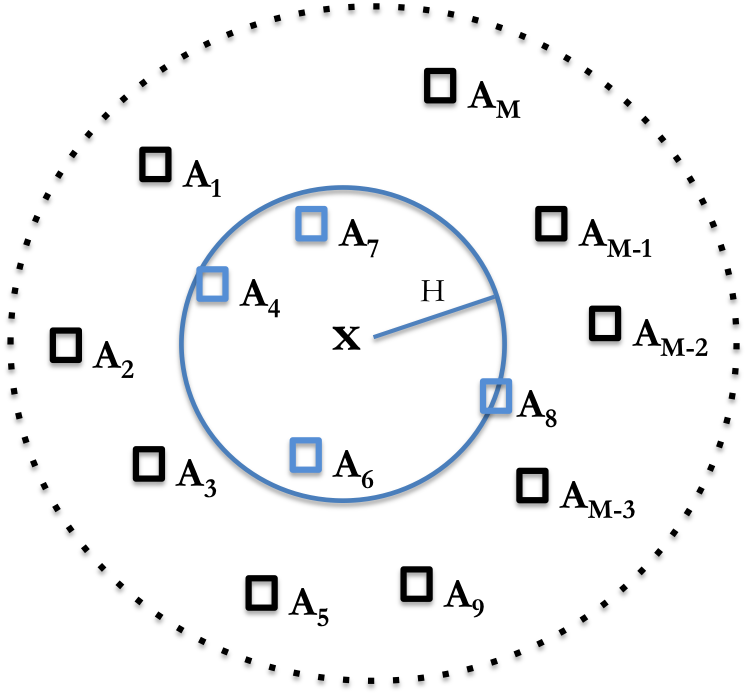
\includegraphics[width=0.29\textwidth]{./figures/sdmOperations.png} &
    \end{tabular}
    \caption{(a) Neural network implementation of a Hopfield
      network. (b) Neural network implementation of an SDM. Both
      networks take binary inputs $\bf{x}_{i}$ of length $N$ and
      produce binary outputs $\bf{z}_{i}$ of length $N$. The Hopfield
      network uses a set of symmetric weights $\bf{T}_{ij}$ and a
      Hebbian learning rule to recover an exemplar from a noisy
      input. The weights between the input and hidden layer in a SDM
      network determine the set of addresses $\bf{a}_{m}$ to read from
      or write to, and the second layer of weights store the contents
      of memory at those addresses. (c) An illustration of the basic
      read/write operations over SDMs. The outer dotted line
      represents the space of $2^{N}$ possible addresses while the
      squares with labels $\bf{A}_{m}$ represent the $M$ sampled hard
      addresses used for storage. The address being requested for
      operation is the $\bf{x}$ in the center of the blue circle of
      radius $H$. The hard addresses selected for operating correspond
      to the blue squares within the Hamming radius of $\bf{x}$.}
\label{neuralNets}
\end{center}
\end{figure}

%%%%%%%%%%%%%%%%%%%%%%%%%%%%%%%%%%%%%%%%%%%%%%
% subsection - SDM
%%%%%%%%%%%%%%%%%%%%%%%%%%%%%%%%%%%%%%%%%%%%%%
\subsection{Sparse Distributed Memory (SDM) systems}

Sparse Distributed Memory (SDM) systems were developed by \citeA{Kanerva1988,Kanerva1993} as a mathematical model of human memory, exploiting the properties of high-dimensional representational spaces.
An SDM can function as an \textit{autoassociative}, \textit{content-addressable} memory (associates a pattern with itself) like a Hopfield network, but can additionally function as a \textit{heteroassociative} memory (associates one pattern with another), and as a \textit{sequential-access} memory (in which a temporal sequence of patterns can be stored and retrieved). A simple way to understand how SDMs work follows from an analogy to conventional computer memory. In typical Random-Access Memory (RAM), bit-words of length $N$ are stored in an array of $M = 2^{N}$ registers. To read from or write data to memory, all that is needed is the data itself (the \textit{contents} of memory), and the location that points to this content (the \textit{address}). This limits the amount of storage in memory (since $M$ is fixed based on the length a word) and the contents in memory have nothing to do with their address in memory (thus one cannot determine the similarity of memory content based their addresses). SDMs were developed to overcome this limitation and to encapsulate the notion that distances between concepts in memory correspond to distances between points in high-dimensional space \cite{Kanerva1988}. Instead of storing and reading data in a sequentially-enumerated set of $M = 2^{N}$ address registers, an SDM considers very bit-words of length $N$ (typically $N > 100$) and samples a very large number $M >> N$ set of hard addresses to use as registers from the space of $2^{N}$ possible addresses. Each point in this sampled space of addresses will be far away from most other points in the sample space (as measured by Hamming distance).

To store a set of binary patterns $\bf{p}^{\alpha}$ of length $N$ in an autoassociative SDM, an address $\bf{a}$ and data $\bf{d}$ must be supplied for each pattern corresponding to a tuple ($\bf{x}^{\alpha}$, $\bf{w}^{\alpha}$), where $\bf{x}^{\alpha}$ = $\bf{w}^{\alpha}$. When acting as a heteroassociative or sequential-access memory system, this equality need not be held. Since the set of $M$ hard addresses does not enumerate the total space of $2^{N}$, a particular address $\bf{x}^{\alpha}$ has high probability of not existing in the sampled addresses space. Thus, existing hard addresses near $\bf{x}^{\alpha}$ are selected for access if they are within a Hamming radius $H$ of $\bf{x}^{\alpha}$, where $H$ represents the number of different bits allowed between points. The contents of these selected addresses are then modified to store the pattern $\bf{w}^{\alpha}$ such that each bit in the contents is increased or decreased by 1 depending on whether or not that bit in the pattern is a 1 or 0, respectively. To read a binary pattern $\bf{z}$ out of memory from address $\bf{x}$, a similar selection procedure is carried out in which a set of hard addresses within a Hamming radius of $\bf{x}$ are accessed, and a bit $j$ in the output $\bf{z}$ is set to 1 or 0 if the sum of the contents in position $j$ over these selected addresses is greater than or less 0, respectively. A neural network implementation of an SDM and an illustrative schematic of an SDM's operation are provided in panels (b) and (c) of Figure \ref{neuralNets} above.

More formally, given a set of binary patterns $\bf{p}^{\alpha}$ of length $N$ in the form ($\bf{x}^{\alpha}$, $\bf{w}^{\alpha}$), an SDM can be constructed as a neural network with $N$ units in the input layer, a hidden layer with $M$ units for each sampled hard addresses, and an output layer with $N$ units. The weights between the input and hidden layer correspond to the $M \times N$ matrix $\bf{A}$ of hard-addresses, and the weights between the hidden and output layer correspond to the $M \times N$ matrix $\bf{C}$ of contents stored at each address. The rule for writing $\bf{w}^{\alpha}$ to memory address $\bf{x}^{\alpha}$ is expressed as:
\begin{align}
 \bf{y}^{\alpha} &= \Theta_{H}(\bf{A}\,\bf{x}^{\alpha}) \\	
 \bf{C} &= \bf{w}^{\alpha}\,\bf{y}^{\alpha} 
\end{align}

\noindent where $\bf{y}^{\alpha}$ is a binary vector of length $M$ with a 1 in position $j$ if hard address $\bf{a}$ is within Hamming distance $H$ of $\bf{x}^{\alpha}$. The rule for reading $\bf{z}$ from memory address $\bf{x}$ is expressed as:
\begin{align}
 \bf{y} &= \Theta_{H}(\bf{A}\,\bf{x}) \\	
 \bf{z} &= g(\bf{C}\,\bf{y}) 
\end{align}
\noindent where $g(x_{i}) = 1$ if $x_{i} > 0$ and $0$ if $x_{i} \leq 0$.  

%%%%%%%%%%%%%%%%%%%%%%%%%%%%%%%%%%%%%%%%%%%%%%%%%%%%%%%%%%%%%%%%%%%%%%
% model evaluation
%%%%%%%%%%%%%%%%%%%%%%%%%%%%%%%%%%%%%%%%%%%%%%%%%%%%%%%%%%%%%%%%%%%%%%
\section{Exemplar storage in associative memory systems}

Having reviewed the formal descriptions of a Hopfield network and an
SDM, we now turn to evaluation of these models using several different
metrics to gauge their fitness as exemplar storage systems. In all
analyses, we used an address length of $N=256$ and, for the SDM, a
Hamming radius of $H=112$.

%%%%%%%%%%%%%%%%%%%%%%%%%%%%%%%%
% subsection - capacity
%%%%%%%%%%%%%%%%%%%%%%%%%%%%%%%%
\subsection{Storage Capacity}

First, we explored the upper bound of storage capacity of the SDM
versus the Hopfield network by generating random, uncorrelated inputs,
storing them in and then retriving them from the different models, and
then observing the amount of corruption introduced during this
procedure. We tested several SDMs with different address space sizes,
$M\in\{500, 1000, 2500, 5000, 10000\}$ (the Hopfield network only has
one address space size, i.e. $M=N$).  Panel (a) in Figure
\ref{fig:capacity} shows the average results of performing this
comparison 100 times for different numbers of stored words. With
sufficiently large $M$, the SDM easily outperforms the Hopfield
network.

The SDM and Hopfield network should be able to work with corrupted
inputs as well. So, we performed the same analysis as above, except
that we attempted to retrieve each exemplar with a corrupted version
of itself and compared the SDM with $M=10000$.  Figure
\ref{fig:capacity} (b) shows these results for different levels of
corruption. At low levels of corruption, the SDM is more resistant to
corrupted inputs than the Hopfield net.

\begin{figure}[h!]
  \begin{center}
    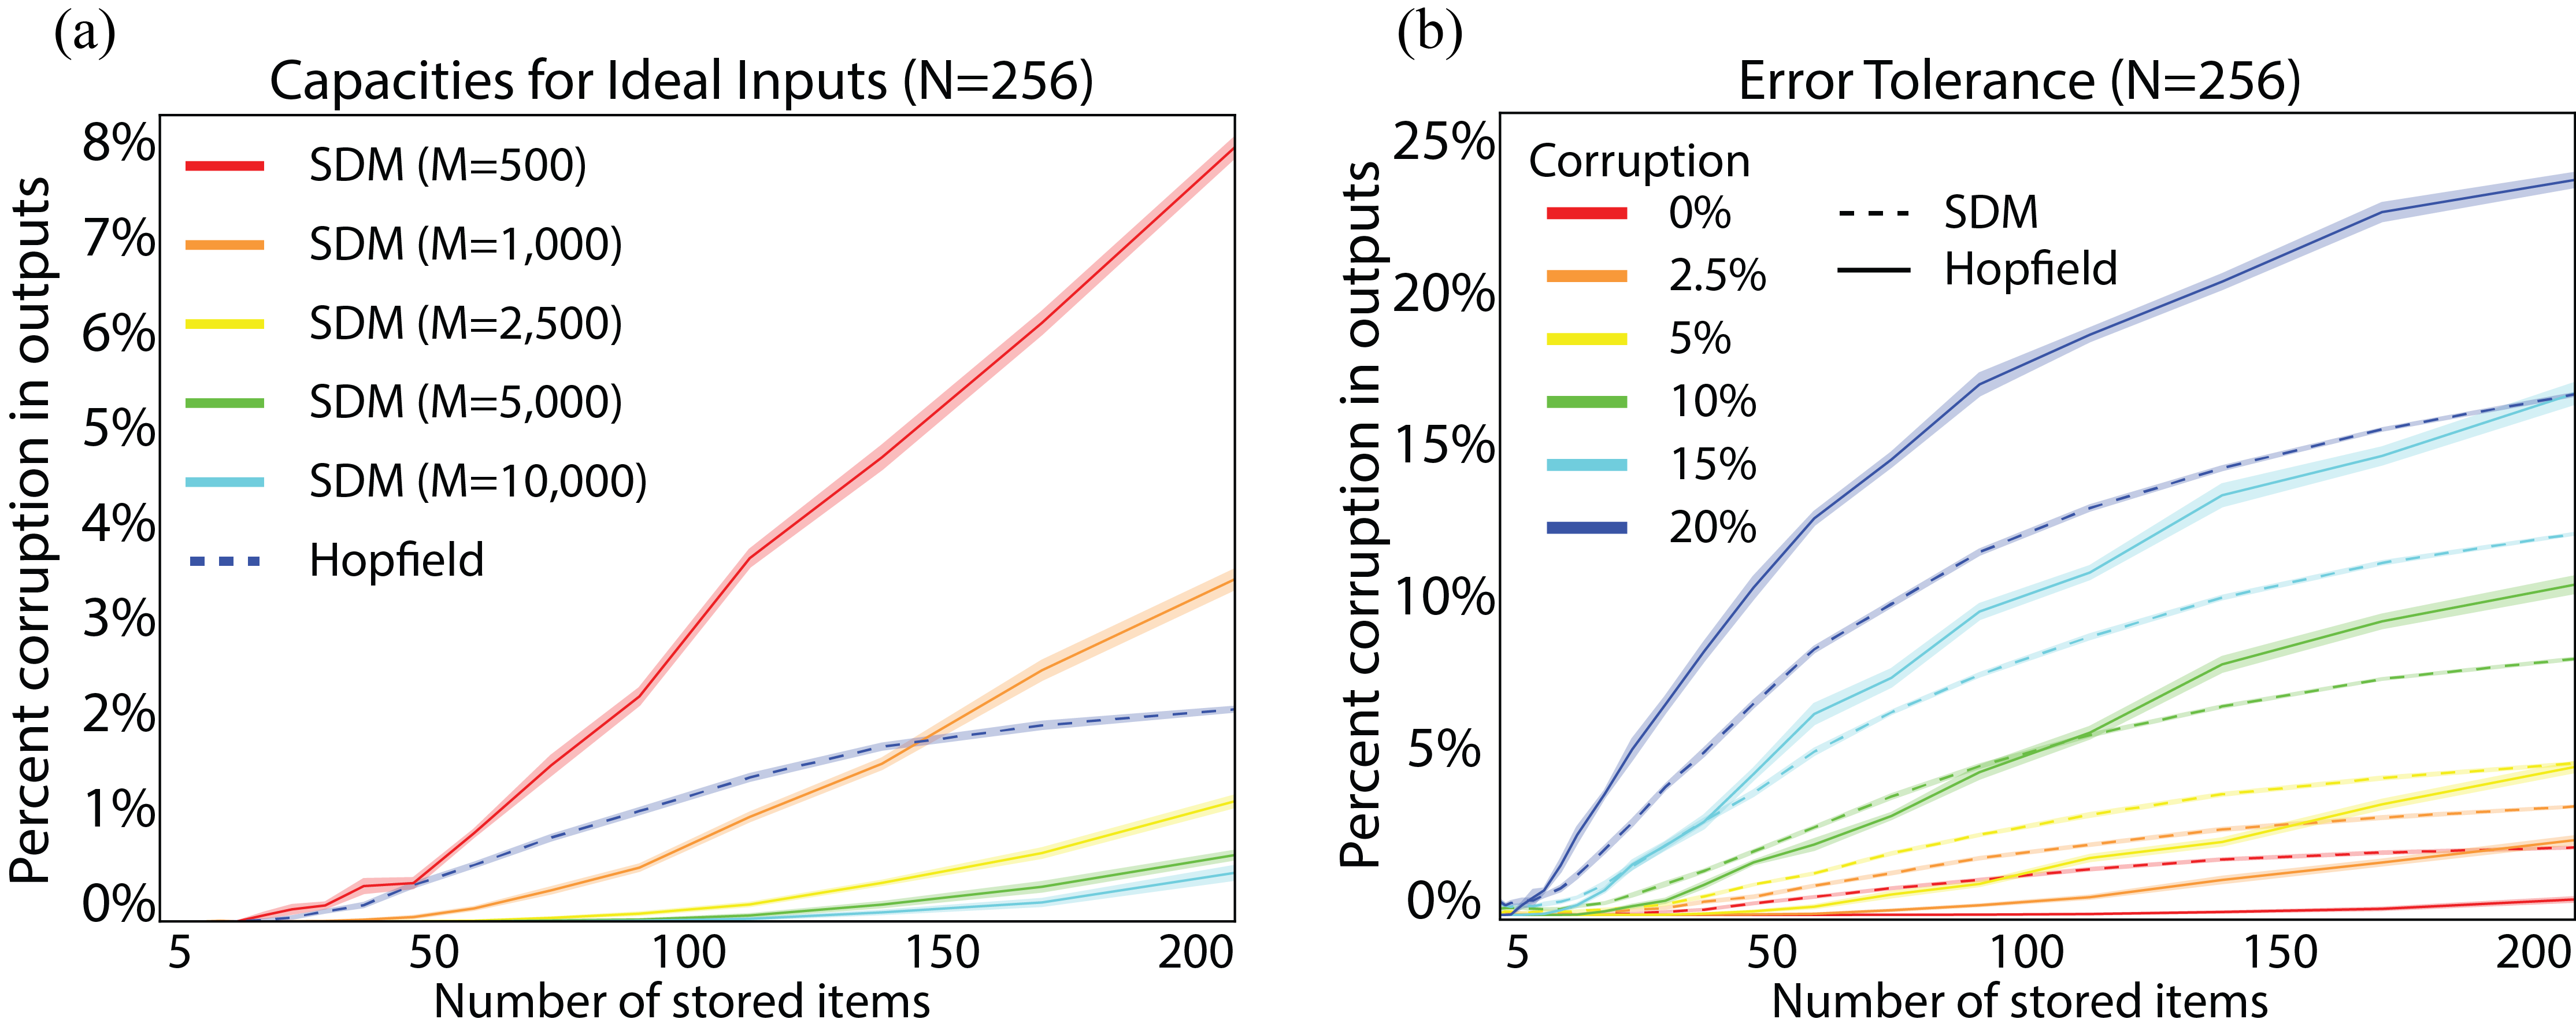
\includegraphics[width=0.9\textwidth]{./figures/all-capacities.png}
    \caption{SDM and Hopfield network capacities. The left plot (a)
      shows the storage capacities of uncorrupted inputs for the
      Hopfield network (dashed line) and SDMs with different address
      space sizes (solid lines). With small address spaces, the SDM
      quickly suffers with relatively high corruption. However, with
      sufficiently large address spaces, the SDM is much more accurate
      than the Hopfield network, being able to store 200 words with
      barely $1\%$ corruption. The right plot (b) shows storage
      capacity when words are read using a corrupted input for
      different levels of corruption.}
    \label{fig:capacity}
  \end{center}
\end{figure}



%%%%%%%%%%%%%%%%%%%%%%%%%%%%%%%%
% subsection - prototypes
%%%%%%%%%%%%%%%%%%%%%%%%%%%%%%%%
\subsection{Prototype Retrieval}


\begin{figure}[t!]
  \begin{center}
    \begin{tabular}{ l l l c}
      \raisebox{2.25in}{(a)} &
      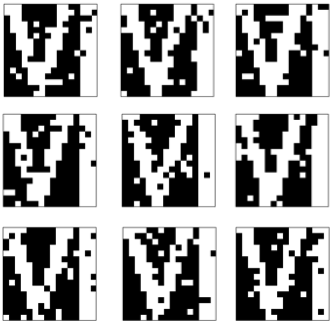
\includegraphics[width=0.38\textwidth]{./figures/exemplars.png} &
      \raisebox{2.25in}{(b)} &
      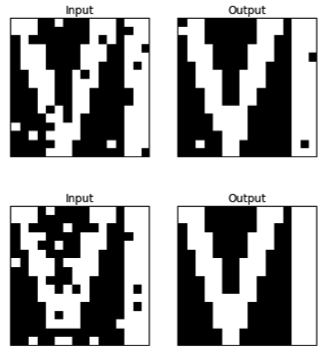
\includegraphics[width=0.36\textwidth]{./figures/prototypeResults.png} \\
      %	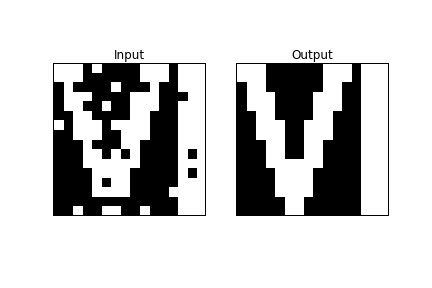
\includegraphics[width=0.4\textwidth]{./figures/vi_sdm.png} 
    \end{tabular}
    \caption{(a) Nine noisy exemplars stored in both SDM and Hopfield
      models. (b) The retrieval results for the Hopfield network (top)
      and SDM network (bottom) when queried with a noisy word.}
    \label{fig:prototypes}
  \end{center}
\end{figure}

\begin{figure}[t!]
  \begin{center}
    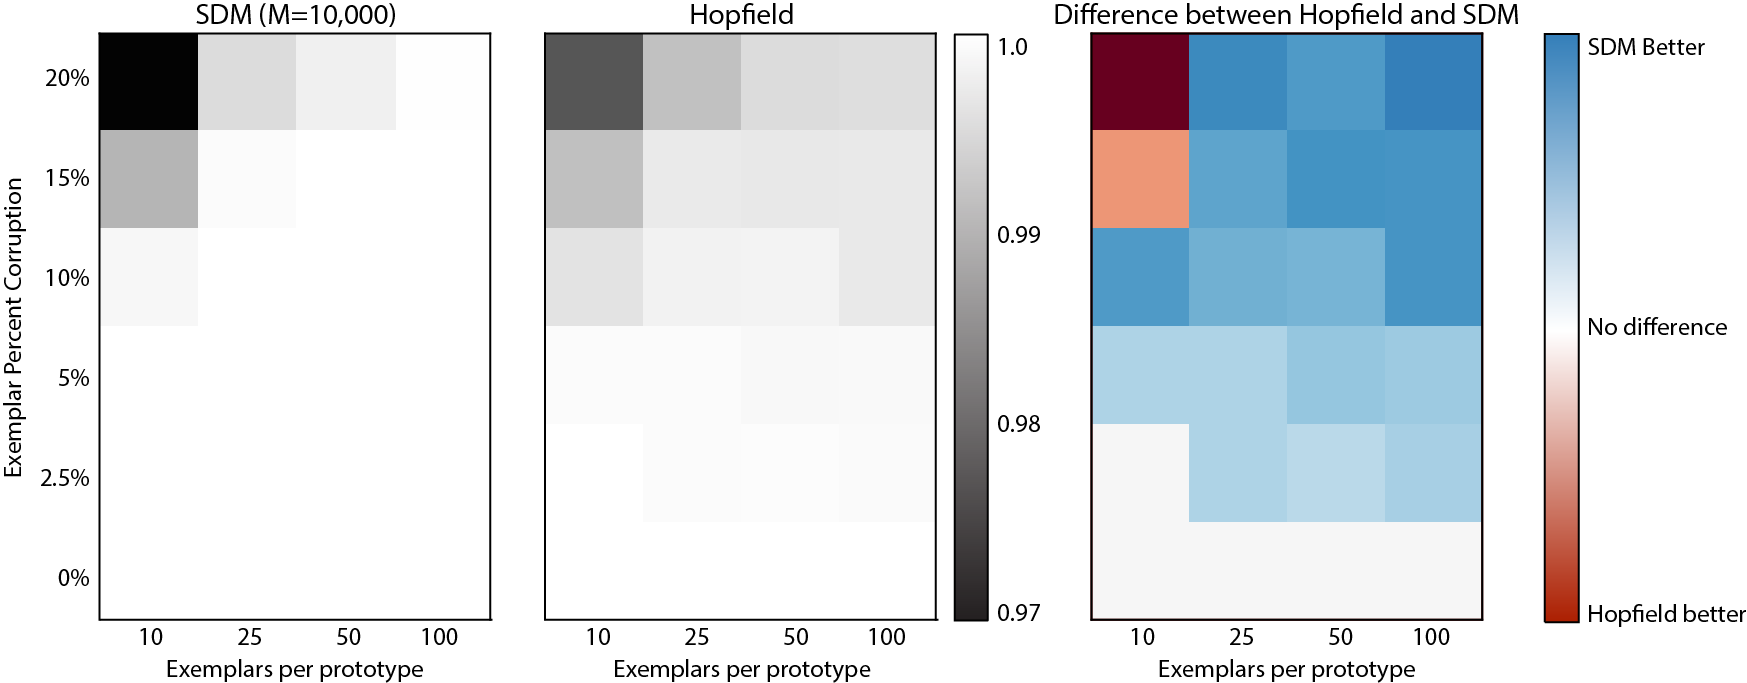
\includegraphics[width=0.87\textwidth]{./figures/prototype-edit.png}
  \end{center}
  \caption{Prototype reconstruction accuracy for the SDM and Hopfield
    network. The left two plots show the accuracy in reconstructing
    three uncorrelated prototypes from different numbers of exemplars
    with different levels of corruption. The right plot shows the
    difference between SDM and Hopfield performance, with white
    indicating no difference, blue indicating better performance by
    the SDM, and red indicating better performance by the Hopfield
    network. In most cases, the SDM outperforms the Hopfield network.}
  \label{fig:prototype-comparison}
\end{figure}

One feature of associative memory systems is the ``averaging'' effect:
as more vectors are stored in the memory, vectors that are close to
each other may overlap in memory and reading will result in a vector
that is somewhere in between. Importantly, this is related to a
property of being able to retrieve a \textit{prototype} vector from
multiple stored \textit{exemplars}. By prototype, we refer to an
unobserved ``ideal'' input. Exemplars are corrupted (or atypical)
observations of this input.

Panel (a) in Figure \ref{fig:prototypes} shows nine exemplars of the
``VI'' roman numeral, each with 25 corrupted bits ($\approx10\%$),
which were stored in the SDM and Hopfield network. Panel (b) in Figure
\ref{fig:prototypes} shows the result of querying each network with
another corrupted exemplar: both return vectors that approach the true
prototype and have much less corruption than any of the exemplars. In
this particular example, the SDM is perfectly able to retrieve the
prototype.

To more rigorously test the abilities of the Hopfield network and SDM
to retrieve prototypes, we performed the following steps 100 times:
first, we generated three uncorrelated prototypes. For each prototype,
we generated several corrupted exemplars, where the Hamming distance
between each exemplar and the prototype was no more than a specified
amount of corruption. We stored these exemplars in the Hopfield
network and SDM ($M=10000$) and then attempted to retrieve the
prototype by querying with a new corrupted exemplar. We computed the
amount of corruption in the prototype, and averaged across the 100
trials. 

Figure \ref{fig:prototype-comparison} shows the results for different
numbers of exemplars and different levels of corruption. Both the SDM
and Hopfield network are able to retrieve near-perfect prototypes for
corruption of no more than $5\%$ (in the case of the SDM, it is
accurate even at $10\%$, consistent with the example in
Figure \ref{fig:prototypes}). At high levels of corruption and low
numbers of exemplars, the Hopfield network actually outperforms the
SDM; however, with more exemplars, the SDM quickly recovers.


% \begin{figure}[t!]
%   \begin{center}
%     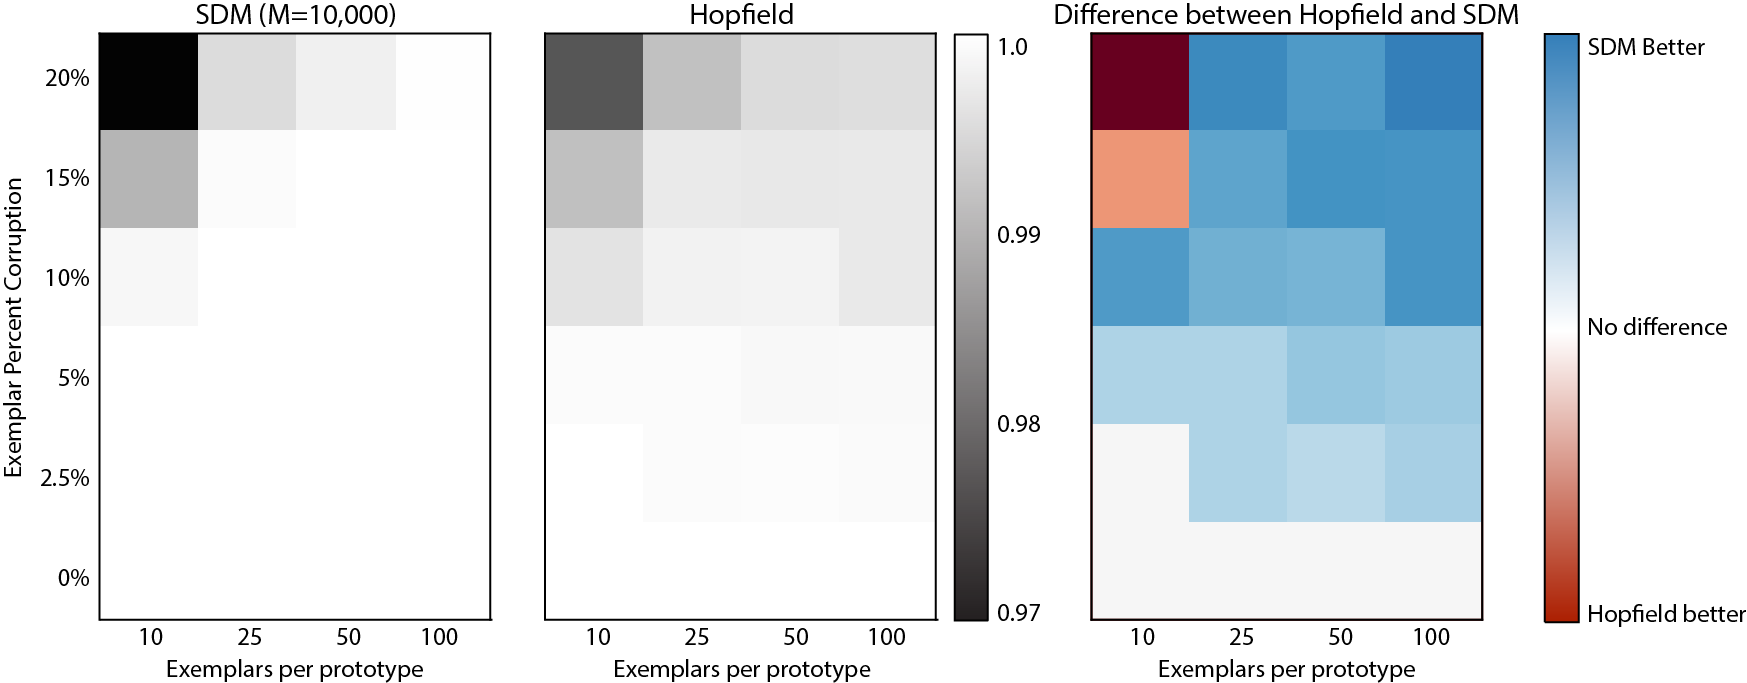
\includegraphics[width=0.95\textwidth]{./figures/prototype-edit.png}
%   \end{center}
%   \caption{Prototype reconstruction accuracy for the SDM and Hopfield
%     network. The left two plots show the accuracy in reconstructing
%     three uncorrelated prototypes from different numbers of exemplars
%     with different levels of corruption. The right plot shows the
%     difference between SDM and Hopfield performance, with white
%     indicating no difference, blue indicating better performance by
%     the SDM, and red indicating better performance by the Hopfield
%     network. In most cases, the SDM outperforms the Hopfield network.}
%   \label{fig:prototype-comparison}
% \end{figure}


%%%%%%%%%%%%%%%%%%%%%%%%%%%%%
% subsection - sequences
%%%%%%%%%%%%%%%%%%%%%%%%%%%%%
\subsection{Sequence Storage}

% just to show off here since the hopnet can't at all - but maybe we should make a comment about recurrent nets (JUST a comment) ?
\begin{figure}[b!]
  \begin{center}
    \begin{tabular}{ l c }
      \raisebox{3.5in}{(a)} &
      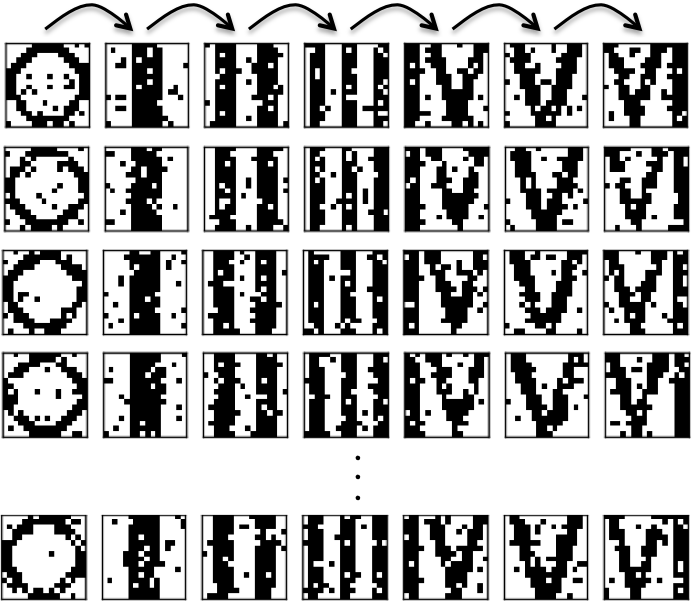
\includegraphics[width=0.7\textwidth]{./figures/exemplarStoredSequences.png} \vspace{25bp} 
      \\
      \raisebox{.55in}{(b)} &
      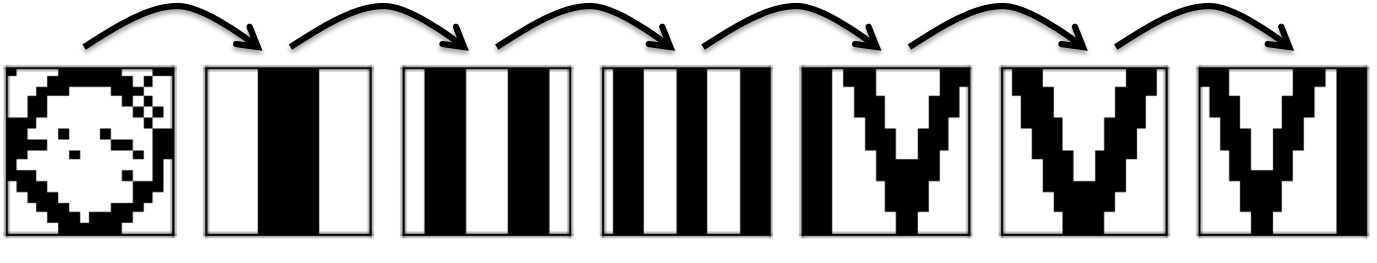
\includegraphics[width=0.7\textwidth]{./figures/prototypeRetrievedSequence.png} 
    \end{tabular}
    \caption{(a) Exemplars of noisy sequences stored in SDM
      memory. (b) Retrieval of prototypical sequence in SDM from a
      noisy word.}
    \label{sequences}
  \end{center}
\end{figure}

Hopfield networks typically function only as autoassociative memory systems, whereas SDMs can associate one pattern with another, acting as a heteroassociative memory. We demonstrate this capability in an SDM by storing and retrieving temporal sequences of patterns.

SDM storage consists of writing and reading binary patterns $\bf{w}^{\alpha}$ at addresses given by $\bf{x}^{\alpha}$. When both pattern and address space consist of the same length of bits, $N$, there are no restrictions prohibiting $\bf{w}^{\alpha}$ to be an address pointing elsewhere in memory. Thus, if one sets $\bf{w}^{\alpha} = \bf{x}^{\alpha+1}$, we can store data as a linked list and retrieve it sequentially. Below in panel (a) of Figure \ref{sequences} we display example sequences of noisy stimuli. Here, each image of a roman numeral (well, technically zero is not a roman numeral) corresponds to a binary pattern of length $256$ and corrupted by $25$ bits ($\approx 10\%$ noise). When writing these patterns to memory, the next numeral's address was stored as the content for the current numeral's address. Consequently, when this SDM is queried with a corrupted numeral, it retrieves the stored sequence of roman numerals following the queried numeral. Furthermore, as shown in panel (b) of Figure \ref{sequences}, these retrieved addresses correspond to the prototype for each numeral stored as an exemplar (in this particular example, there were $10$ noisy sequences stored in an SDM with $M=10000$).




%%%%%%%%%%%%%%%%%%%%%%%%%
% subsection - discussion
%%%%%%%%%%%%%%%%%%%%%%%%%
\subsection{Discussion}

To summarize, we compared the SDM and the Hopfield network on storage
capacity for uncorrupted and corrupted inputs and on prototype
retrieval. In most cases, the SDM outperformed the Hopfield
network. Interestingly, however, is the capacity when retrieving with
corrupted inputs or prototype retrivel. At higher levels of noise, the
SDM is actually more error-prone than the Hopfield network in these
scenarios. We suspect this is due to an overlap between the corrupted
input and the Hamming radius of a different stored word. More
specifically, if we flip exactly $b$ bits, then the word will be
located along an edge in space that is $b$ bits away from the actual
stored word in Hamming distance. At $20\%$ corruption, the Hamming
radius for activating addresses is approximately $2b$. Thus, although
the Hamming radius of one word does not include another word, it is
not unlikely that that radius will overlap the ``corruption radius'';
thus resulting in a retrieved vector that is somewhere in between the
two stored words.

Because the SDM has poor performance at high levels of noise, it is
less ideal than the Hopfield network when storing only one version of
each word. If a sufficient number of exemplars can be stored, however,
it the SDM is clearly superior: with enough exemplars, it can almost
perfectly reconstruct a prototype, whereas the Hopfield net will
always result in some corruption regardless of the number of
prototypes.

A further benefit of the SDM over the Hopfield network is its ability
to store sequences. This is the result of an important property of the
SDM, which is that it can function as a \textit{heteroassociative}
memory, where \textit{address} and \textit{content} do not need to be
the same. Hopfield networks do not have this capability, and therefore
are limited in the data structures they can store.

One downside of the SDM is that it is less efficient than the Hopfield
network. We used an address space size of 10000, which is not
atypical. With such a large address space, however, comes a large
computational overhead. However, if memory and computation are not an
issue, then the SDM is clearly a better choice over the Hopfield
network: it is for the most part more accurate, it has a higher
capacity, and it is capable of much more sophisticated behavior than
the Hopfield network.


%%%%%%%%%%%%%%%%%%%%%%%%%%%%%%%%%%%%%%%%%%%%%%%%%%%%%%%%%%%%%%%%%%%%%%
% future directions
%%%%%%%%%%%%%%%%%%%%%%%%%%%%%%%%%%%%%%%%%%%%%%%%%%%%%%%%%%%%%%%%%%%%%%
\section{Probabilistic interpretations of SDMs}

Exemplar models have more potential than uniformly storing data and
recovering its mean. \citeA{Shi2010} demonstrated that exemplar models
can be used to implement \textit{importance sampling}, a Monte Carlo
method of approximating Bayesian inference.  Can SDMs be used to
implement importance sampling? Previous work has formalized a
probabilistic interpretation of SDMs \cite{Anderson1989}, thus
suggesting that it should be possible to adjust that formalization to
specifically encompass exemplar-based approximate inference. Here, we
extend the idea of using exemplar models for importance sampling in
the context of SDMs.

\subsection{Overview}

In general, our goal is to use SDMs to recover the expectation of some
function $f(x^*)$. However, we cannot directly observe $x^*$; instead,
we have observations $x$. Importance sampling provides a way for us to
infer the value of $x^*$ given our observations, and therefore compute
$y$. This is given by Eq. 12 in \citeA{Shi2010}:
\begin{equation}
E[f(x^*)|x]\approx \frac{\sum_j f(x_j^*)\Pr(x|x_j^*)}{\sum_j \Pr(x|x_j^*)}
\end{equation}

To translate this into the context of a SDM, let $x^*$ be the
uncorrupted target address at which we want to read or write a value
$y$. If $x$ is a corrupted version of $x^*$, then we wish to choose
some addresses $a_j$ given $x$ such that reading and writing to those
addresses approximate reading and writing $(x^*,y)$. This is
equivalent to computing the expectation of $f(x^*)=y$ over the
addresses $a_j$.

\subsection{Writing}

Let us define the probability of writing to address $a_j$ given an
input address $x_i^*$ as $w(a_j|x_i^*)$. In the limit, the number of
addresses increases to the point where we will always be able to write
to exactly $x_i^*$. Thus, this writing density must satisfy the
following constraint:
\begin{equation}
\lim_{M\rightarrow 2^N}w(a_j|x_i^*) = \delta(a_j=x_i^*)
\label{eq:w}
\end{equation}

\noindent After writing multiple values $(x_i^*, y)$, the value of the counter
associated with address $a_j$ will be:
\begin{equation}
C_j=\sum_i w(a_j|x_i^*)y_i
\label{eq:Cj}
\end{equation}

\subsection{Reading}

We are given an address $x$, which as before is a corrupted version of
$x^*$; the goal is to read the value stored at $x^*$. We can define a
reading density as the likelihood that $x$ was generated from some
$a_j$:
\begin{equation}
r(x| a_j)\propto \Pr(x|x^*=a_j)
\label{eq:r}
\end{equation}

\noindent We weight the counter value $C_j$ for each $a_j$ based on the
likelihood that $a_j$ is the actual target address. The sum over these
values is:
\begin{equation}
f(x)=\sum_j C_j r(x| a_j)
\label{eq:R}
\end{equation}

% \begin{equation}
% R(x) = 
% \end{equation}

\noindent The expected value of this sum over all addresses $a$ is obtained by
substituting Eq. \ref{eq:Cj} into Eq. \ref{eq:R} and simplifying according
to linearity of expectation:
\begin{align}
\mathbb{E}_a[f(x)]&=\mathbb{E}_a\left[\sum_j\left(\sum_i w(a_j| x_i^*)y_i\right)r(x|a_j)\right]\\
&=\sum_i\ y_i\cdot E_a\left(\sum_j w(a_j| x_i^*)r(x|a_j)\right)
\end{align}

\noindent As our address space grows larger (as in Eq. \ref{eq:w}), this approaches:
\begin{align}
\lim_{M\rightarrow 2^N} \mathbb{E}_a[f(x)]&=\sum_i\ y_i \int_a \delta(a-x_i^*)\Pr(x|x^*=a)\ \mathrm{d}a\\
&= \sum_i\ y_i\Pr(x|x_i*)
\end{align}

\noindent Thus, in the limit, the expected value that we read out will be:
\begin{equation}
\mathbb{E}[y|x]\propto \sum_i\ y_i\Pr(x|x_i^*)
\end{equation}

% \subsection{Empirical comparison}

% To verify this formulation of the SDM as an importance sampler, we
% \\

%%%%%%%%%%%%%%%%%%%%%%%%%%%%%%%%%%%%%%%%%%%%%%%%%%%%%%%%%%%%%%%%%%%%%%
%  conclusions
%%%%%%%%%%%%%%%%%%%%%%%%%%%%%%%%%%%%%%%%%%%%%%%%%%%%%%%%%%%%%%%%%%%%%%
\section{Conclusions and Future Work}

In this paper, we compared two associative memory systems: Hopfield
networks and Sparse Distributed Memory (SDM). We found that the SDM
was largely superior to Hopfield networks in terms of storage
capacity, error tolerance during retrieval, and accuracy in prototye
reconstruction. Moreover, the SDM is capable of storing complicated
data structures -- such as linked lists -- due to its separation of
addresses and contents.  These structures are not possible in Hopfield
networks, which do not separate contents from addresses. Thus, given a
choice of associative memory, SDMs seem the clear victor.

Given the robustness of SDMs, we took them one step further and
explored their potential to be used for Bayesian
inference. Associative memory is conducive to exemplar storage, and
exemplar models have previously been shown to approximate Bayesian
inference via importance sampling \cite{Shi2010}. Thus, SDMs should
similarly be able to perform importance sampling. We formalized this
notion mathematically, laying a foundation for future work which will
empirically test SDM importance samplers. In particular, this will
involve an investigation into the choice of a likelihood function. An
immediate question is: is it possible to find an encoding of the data
into binary vectors which results in an approximation that is
equivalent to the approximation obtained by changing the likelihood
function? If it is, this would make importance sampling in a SDM much
more flexible and generic by not requiring a change in read
probabilities.

Another area of future work is quantifying the extent to which
corruption hinders the SDM. We found that in certain cases --
particularly when the amount of corruption in the input is high -- the
SDM has poorer accuracy than the Hopfield network. We provided an
explanation for why this might be, but a more rigorous exploration of
such phenomena is necessary to understand the SDM's computational
constraints.

Through this project, we have made several contributions to the
understanding of associative memory and its interface with
computational-level models. Our first contribution was to motivate a
rational algorithmic-level model of exemplar memory using associative
networks. Our second contribution was to empirically compare two
associative memory systems, Hopfield networks and SDMs, as models for
exemplar storage. Finally, our third contribution was to
mathematically formalize a form of approximate Bayesian inference --
importance sampling -- in the context of the SDM. We believe the SDM
is a promising framework for exploring rational process models and
look forward to future collaborations with the Redwood Neuroscience
Institute extending the work presented here.

%%%%%%%%%%%%%%%%%%%%%%%%%%%%%%%%%%%%%%%%%%%%%%%%%%%%%%%%%%%%%%%%%%%%%%
% bibliography
%%%%%%%%%%%%%%%%%%%%%%%%%%%%%%%%%%%%%%%%%%%%%%%%%%%%%%%%%%%%%%%%%%%%%%

%\newpage
\bibliographystyle{apacite}

\setlength{\bibleftmargin}{.125in}
\setlength{\bibindent}{-\bibleftmargin}

\bibliography{classProject}


% %%%%%%%%%%%%%%%%%%%%%%%%%%%%%%%%%%%%%%%%%%%%%%%%%%%%%%%%%%%%%%%%%%%%%%
% % appendix (code)
% %%%%%%%%%%%%%%%%%%%%%%%%%%%%%%%%%%%%%%%%%%%%%%%%%%%%%%%%%%%%%%%%%%%%%%
% \newpage
% \appendix

% \section{Project Code}
% This is where we have the code.


\end{document}
